\documentclass[a4paper, 12pt]{report}

%% Pour des marges plus équitables.
\usepackage[margin=2cm]{geometry}
%% Pour la langue des titres et sous-titres.
\usepackage[francais]{babel}
%% Pour de belles images.
\usepackage{graphicx}
%% Pour la police de caractères.
\usepackage{fontspec}
%% Pour les liens externes.
\usepackage{hyperref}

\setmainfont{Sansation Light}

\begin{document}
\begin{titlepage}
	\vspace*{\fill}
	\begin{center}
		{\Huge Thésaurus, l'analyse}\\
		\vspace{\fill}
		Franck Petitdemange \\
		Nordine El Hassouni \\
		Issam Amal \\
		Cyril Monmouton \\
		Marouane Denguiri \\
		Mohamed Amine Zahir \\
		Abdelhamid Belarbi
	\end{center}
	\vspace*{\fill}
	\center{\today}
\end{titlepage}

\tableofcontents

\begin{chapter}{Genèse}
	\begin{section}{Le groupe et le sujet}
		Le groupe est constitué des sept personnes nommées sur la page de garde et le responsable du projet est Abdelhamid Belarbi
		\footnote{Élu démocratiquement à 71,42 \% des voix.}.\\
		Nous avons choisi de traiter le thème de l’\emph{astronomie} au sens large du terme. Nous inclurons donc des termes tels que \emph{Comète},
		\emph{Galaxie}, \emph{Étoile} ou bien \emph{Voie Lactée}.
	\end{section}
	
	\begin{section}{Définitions}\label{aspic}
		Internet regorge de définitions de thésaurus et des notions qui s’y rapportent (voir \cite{Wikipedia}, \cite{Inpes}, \cite{Bdsp} et \cite{Unesco}).
		Toutefois, beaucoup d’entre elles sont peu claires, très vagues voire obscures. En tant que concepteurs d’une application, nous nous devions de réunir les
		meilleures définitions, les clarifier et les spécifier sans ambiguïté.\\
		
		
		
		\noindent
		Nous utiliserons les définitions suivantes.
		\begin{subsection}{Définitions globales}
			\begin{description}
				\item[\emph{Terme} :] mot ou combinaison de mots significatifs.
				\item[\emph{Descripteur} :] terme choisi pour caractériser les informations, aide à l'indexage et la recherche (= terme préférentiel ou vedette).
				\item[\emph{Non-descripteur} :] terme non accepté à l'indexation, il peut s'agir de synonyme, abréviation ou variante orthographique d'un descripteur
				(= terme non préférentiel ou
				synonyme).
				\item[\emph{Microthésaurus} :] ensemble de descripteurs reliés au même concept. Noté \emph{MT}.
				\item[\emph{Thésaurus} :] ensemble de micro-thésaurus.
			\end{description}
		\end{subsection}
		
		\begin{subsection}{Pour les relations entre termes}
			\label{glouglou}
			\begin{description}
				\item[\emph{EP (Employé Pour)} :] relation entre un descripteur et le (ou les) non-descripteur qu'il référence.
				\item[\emph{EM (Employer)} :] relation entre un non-descripteur et son descripteur (symétrique de la relation précédente).
				\item[\emph{TA (Terme Associé)} :] relation entre des descripteurs appartenants à des micro-thésaurus différents, mais entre lesquels peuvent exister des
				proximités sémantiques.
				\item[\emph{TS (Terme Spécifique)} :] relation entre un descripteur plus général et un (ou plusieurs) descripteur plus spécifique.
				\item[\emph{TG (Terme Général)} :] relation entre un descripteur plus spécifique et un descripteur plus général (symétrique de la relation précédente).
			\end{description}
		\end{subsection}
		
		\begin{subsection}{Pour les modes d'indexation}
			\begin{description}
				\item[\emph{Liste alphabétique structurée} :] Les descripteurs sont affichés par ordre alphabétique avec leur relations sémantiques.
				\item[\emph{Liste par micro-thésaurus} :] Les descripteurs sont affichés hiérarchiquement, du plus général au plus spécifique.
				\item[\emph{Liste alphabétique permutée} :] Les termes sont affichés selon les notions dans lesquelles ils apparaissent.
			\end{description}
		\end{subsection}
	\end{section}
\end{chapter}

\begin{chapter}{Analyse}
	\begin{section}{Spécifications}
		Les fonctionnalités que nous voulons faire figurer dans l'application sont les suivantes :
		\begin{itemize}
			\item Recherche par mot clé sur l'ensemble des descripteurs;
			\item Affichage du thésaurus indexé des trois manières possibles;
			\item Interface d'administration permettant d'ajouter et de manipuler des termes.
		\end{itemize}
		
		Ces différentes fonctionnalités sont décrites plus en détail dans le diagramme suivant.
	\end{section}
	\begin{section}{Diagramme Use-Case}\label{re}
		\begin{figure}[h]
			\label{sucresale}
			\begin{center}
				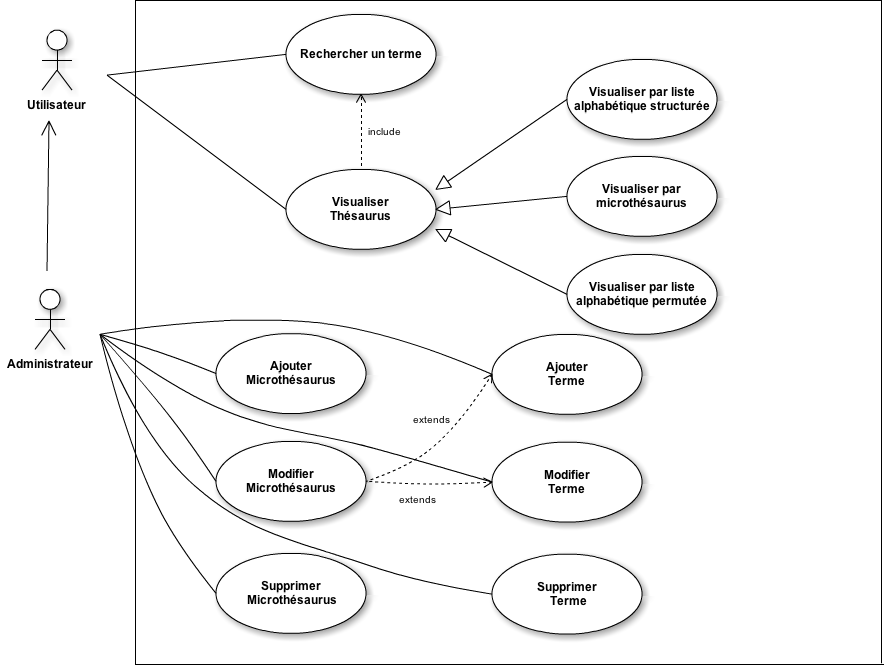
\includegraphics[width=15cm]{Use-Case.png}
				\caption{Le diagramme des cas d'utilisation}
			\end{center}
		\end{figure}~\\
		
		\begin{subsection}{Analyse textuelle}
			Quelques précisions s'imposent quant au diagramme précédent.\\
			\begin{itemize}
				\item L'utilisateur est un simple visiteur anonyme.
				\item La recherche s'effectue en spécifiant un mot-clé et un mode d'affichage (d'indexation).
				\item Visualiser un thésaurus revient soit à le voir en entier avec tout les termes de la base,
					soit un seul micro-thésaurus, soit un seul terme avec tous les termes auxquels il est lié.
				\item Lorsque l'administrateur ajoute ou modifie un terme, il peut spécifer le micro-thésaurus auquel il appartient d'où les flèches \emph{<<extends>>}.
			\end{itemize}
		\end{subsection}
	\end{section}
	
	\begin{section}{Diagramme des classes}
		\begin{figure}[h]
			\label{classeur}
			\begin{center}
				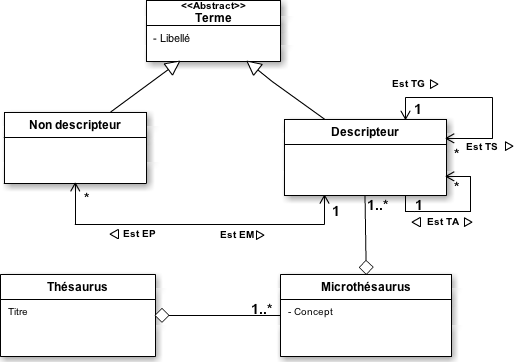
\includegraphics[width=13cm]{Classes.png}
				\caption{Le diagramme des classes}
			\end{center}
		\end{figure}~\\
		
		Le diagramme parle de lui-même. Toutes les définitions données dans la section \ref{aspic} sont appliquées, d'où l'utilité de la démarche de clarification
		effectuée.\\
	\end{section}
\end{chapter}



%% Sitographie
\renewcommand\bibname{Webographie}%% Changement du titre de bibliographie en webographie.
\begin{thebibliography}{2}
	\bibitem{Wikipedia}
	L'encyclopédie que l'on ne présente plus, utile pour les définitions.\\
	\emph{Adresse} : \url{fr.wikipedia.org}
	~\\
	\bibitem{Inpes}
	Un thésaurus très bien fait qui est présenté dans les trois modes d'indexation.\\
	\emph{Alphabétique structuré} : \url{www.inpes.sante.fr/30000/pdf/thesaurus/thes\_01.pdf}\\
	\emph{Microthésaurus} : \url{www.inpes.sante.fr/30000/pdf/thesaurus/thes\_02.pdf}\\
	\emph{Alphabétique permuté} : \url{www.inpes.sante.fr/30000/pdf/thesaurus/thes\_03.pdf}
	~\\
	\bibitem{Bdsp}
	Le (très) gros thésaurus de la Banque de données en Santé Publique, très instructif.
	\emph{Adresse} : \url{asp.bdsp.ehesp.fr/Thesaurus/}
	~\\
	\bibitem{Unesco}
	Le thésaurus de l'Unesco, une autre aide précieuse pour bien comprendre les principes.
	\emph{Adresse} : \url{databases.unesco.org/thesfr/}
	~\\
	\bibitem{Oracle SQL reference}
	La documentation Oracle officielle pour faire du SQL dans les normes.
	\emph{Adresse} : \url{docs.oracle.com/cd/E11882_01/server.112/e26088/toc.htm}
\end{thebibliography}
\end{document}
